\section{Simulation Analysis}
\label{sec:simulation}


%Introduzir a cena do ngspice costume
%Mostrar a cena optimizada e explicar o porque de termos usado estes valores diferentes

\indent
 
 This section discusses the circuit simulation, performed using {\it Ngspice}. 

This circuit was entered into the {\it Ngspice} simulation environment. This tool is used to simulate analog electronic circuits and predict circuit behaviour. 

After having the base circuit description, the parameters have been chosen by trial and error. The final values are present on the following table (table \ref{tab:InputParam}):

\begin{table}[H]
  \centering
  \begin{tabular}{|l|r|}
    \hline    
    {\bf Name} & {\bf Value} \\ \hline
    \input{../Analysis/inputs.tex}
  \end{tabular}
  \caption{Input Parameters}
  \label{tab:InputParam}
\end{table}


In this iterative progress, we arrived at these conclusions about each main parameter:
 
\begin{itemize}
    \item\textbf{Effect of the Coupling Capacitors:}
    The coupling capacitor's main purpose is to neglect any constant current values in order to ensure that the transistors are always in F.A.R.. A consequence that may come from this is the blocking of some low frequencies, lowering therefore the bandwidth.

    \item\textbf{Effect of the Bypass Capacitor:}
    The bypass capacitor $C_b$ is used in order to neutralize the negative impact that the resistor $R_e$ has on the gain. By putting both components in parallel, the capacitor works as a bypass neglecting the effect that the resistor has on the gain when the current is AC.  Meanwhile, when the current is DC, it acts as an open-circuit, allowing the resistor to do its job.
 
    \item\textbf{Effect of the Resistor $R_C$:}
    The resistor $R_C$ has a direct influence in the current $I_C$ which in turn determines the value of $g_m$. This value directly influences the gain. In summary the gain increases when $R_C$ increases and vice-versa.
\end{itemize}    

 


\subsection{Results}

\indent

With the parameters honed in, the OP analysis was possibly, visible on table \ref{tab:OP_ngs}:

\begin{table}[H]
  \centering
  \begin{tabular}{|l|r|}
    \hline    
    {\bf Name} & {\bf Value} \\ \hline
    @c[i] & 0.000000e+00\\ \hline
@gcs[i] & -2.04136e-04\\ \hline
@r1[i] & 1.945229e-04\\ \hline
@r2[i] & -2.04136e-04\\ \hline
@r3[i] & -9.61363e-06\\ \hline
@r4[i] & 1.156284e-03\\ \hline
@r5[i] & 2.041365e-04\\ \hline
@r6[i] & 9.617613e-04\\ \hline
@r7[i] & 9.617613e-04\\ \hline
v(1) & 5.008942e+00\\ \hline
v(2) & 4.808960e+00\\ \hline
v(3) & 4.394159e+00\\ \hline
v(4) & 0.000000e+00\\ \hline
v(5) & 4.837862e+00\\ \hline
v(6) & 5.474755e+00\\ \hline
v(7) & -2.00872e+00\\ \hline
v(8) & -2.97092e+00\\ \hline

  \end{tabular}
  \caption{OP Analysis}
  \label{tab:OP_ngs}
\end{table}

With a few calculations, it is possible to obtain the different values for the voltage across the terminals of both transistors:

\begin{table}[H]
  \centering
  \begin{tabular}{|l|r|}
    \hline    
    {\bf Name} & {\bf Value} \\ \hline
    @gcs[i] & -2.04136e-04\\ \hline
@r1[i] & 1.945229e-04\\ \hline
@r2[i] & -2.04136e-04\\ \hline
@r3[i] & -9.61363e-06\\ \hline
@r4[i] & 1.156284e-03\\ \hline
@r5[i] & 2.041359e-04\\ \hline
@r6[i] & 9.617613e-04\\ \hline
@r7[i] & 9.617613e-04\\ \hline
v(1) & 5.008942e+00\\ \hline
v(2) & 4.808960e+00\\ \hline
v(3) & 4.394159e+00\\ \hline
v(4) & 0.000000e+00\\ \hline
v(5) & 4.837862e+00\\ \hline
v(6) & 5.474753e+00\\ \hline
v(7) & -2.00872e+00\\ \hline
v(8) & -2.97092e+00\\ \hline

  \end{tabular}
  \caption{OP analysis deep dive}
  \label{tab:OP2_ngs}
\end{table}

As it can be seen, the differences are positive, which means that the voltage across the terminals is greater than the saturation voltage of the transistors, which in turn ensures that they are on the F.A.R..

After the OP analysis, it is possible to perform a frequency analysis, that can be seen on the next 2 graphs (Figure \ref{fig:FreqANGS}):

\begin{figure}[H]
\centering
\begin{subfigure}{.5\textwidth}
  \centering
  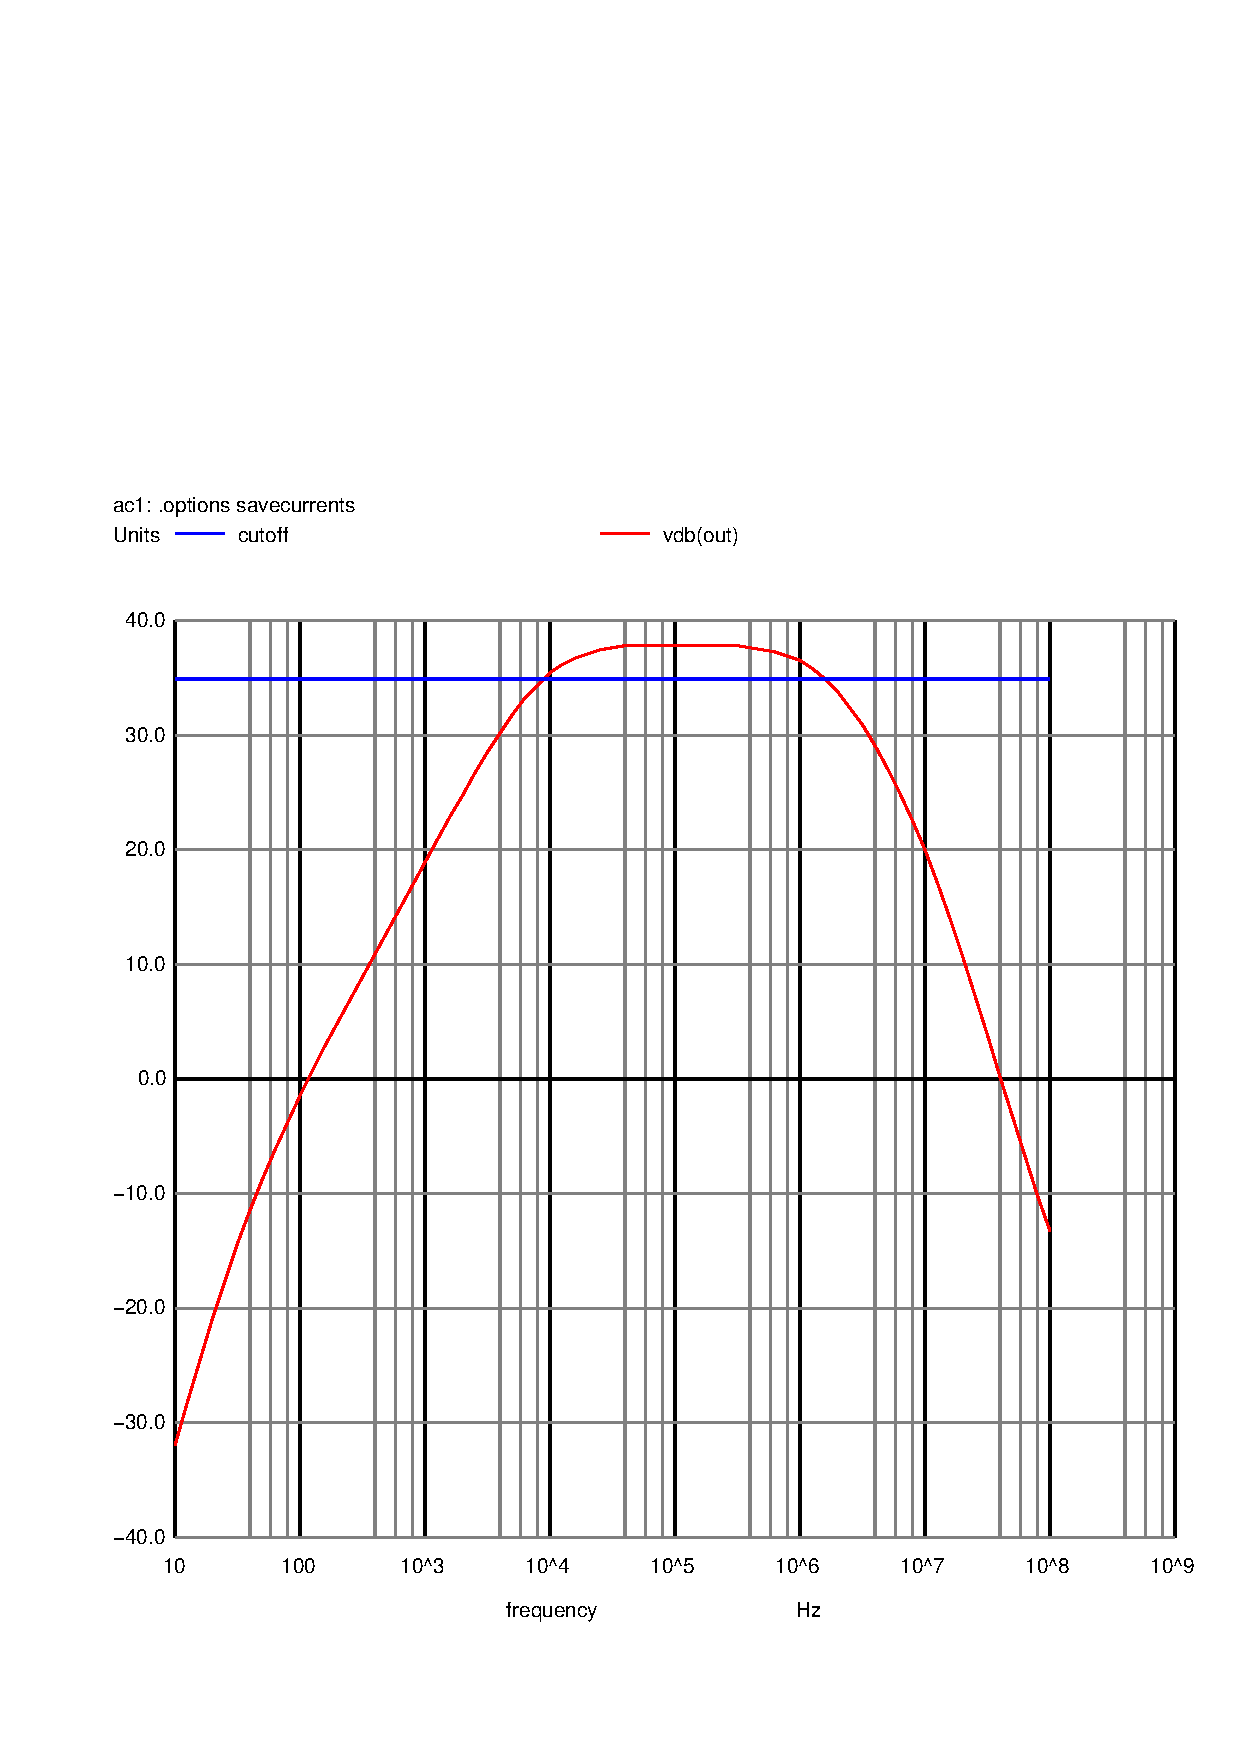
\includegraphics[width=.8\linewidth, trim={2cm 1.5cm 0.5cm 6cm}, clip]{../Simulation/vo2f_m.pdf}
  \caption{Magnitude}
\end{subfigure}%
\begin{subfigure}{.5\textwidth}
  \centering
  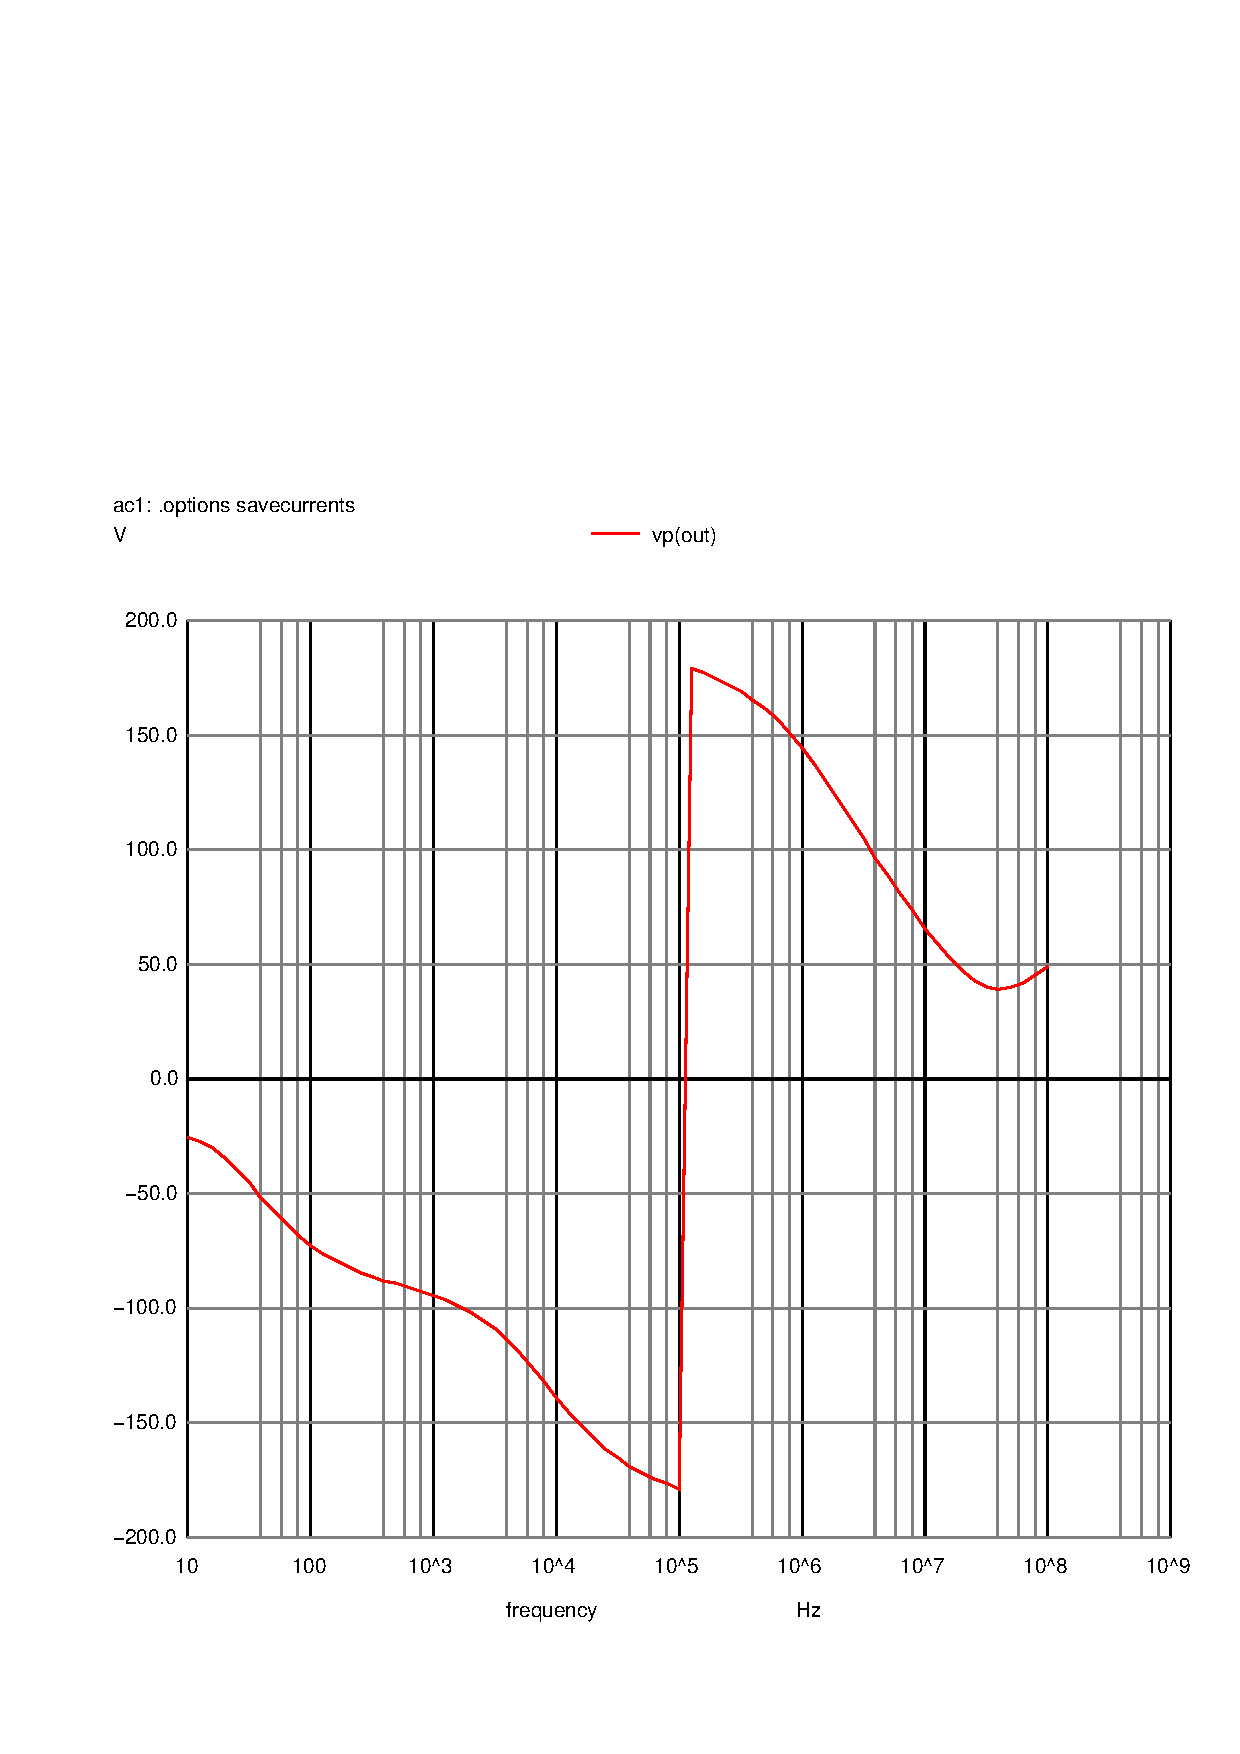
\includegraphics[width=.8\linewidth, trim={2cm 1.5cm 0.5cm 6cm}, clip]{../Simulation/vo2f_ph.pdf}
  \caption{Phase}
\end{subfigure}
\caption{Frequency analysis}
\label{fig:FreqANGS}
\end{figure}


With this done, the final parameter for the Audio amplifier can be obtained:

\begin{table}[H]
  \centering
  \begin{tabular}{|l|r|}
    \hline    
    {\bf Name} & {\bf Value} \\ \hline
    \input{../Simulation/freq_tab.tex}
  \end{tabular}
  \caption{Output parameters}
  \label{tab: OutputParamNGS}
\end{table}

As we can see, the impedances match what we expectected: the output impedance is low and similar to the resistance of the load, wheras the input impedance is high, which is desirable.


Finally, since there is no visible distortion on the next graph, it is possible to ensure that the signal is correctly amplified.


\begin{figure}[h!]
    \centering
  \includegraphics[width=.6\linewidth, trim={2cm 1.5cm 0.5cm 6cm}, clip]{../Simulation/vout.pdf}
  \caption{Transient analysis - Voltage output}
  \label{tab:TransNGS}
\end{figure}


As shown, the signal is greatly amplified and shows no visible distortions. One possible downside of this approach is that the phase of the output is not the same as the phase of the input. However, this is not a problem since the human ear is not sensible enough to notice it.
